% Public arXiv showcase of the manuscript.
% Editorial baseline: Elsevier / Computers & Industrial Engineering (CIE).
% Single-file source in this folder; references resolved through artigos_icpr.bib.
% Operational notes checked against the CIE guide on 2026-03-15:
% - Abstract: concise and factual, maximum 250 words.
% - Keywords: 1 to 7, in English.
% - Highlights for a future submission: 3 to 5 bullet points, each with at most
%   85 characters including spaces; see highlights.txt.
% - Graphical abstract: optional.
% - No explicit page limit or body word limit was identified in the current
%   CIE guide. The manuscript should therefore follow journal-style completeness
%   rather than conference-style compression.
% - Article text should be organized in clearly defined and numbered sections.
% - References should follow APA style.
\documentclass[preprint,12pt,number,longtitle]{elsarticle}

\usepackage[T1]{fontenc}
\usepackage[utf8]{inputenc}
\usepackage{array}
\usepackage{booktabs}
\usepackage{float}
\usepackage{graphicx}
\usepackage{longtable}
\usepackage[section]{placeins}
\usepackage{tabularx}
\usepackage[table]{xcolor}
\usepackage{url}
\usepackage{xurl}
\usepackage[hidelinks]{hyperref}

\journal{Computers \& Industrial Engineering}
\graphicspath{{figures/}}
\biboptions{sort&compress}
\def\UrlFont{\rmfamily}
\pdfstringdefDisableCommands{\def\corref#1{}}
\newcolumntype{Y}{>{\raggedright\arraybackslash}X}
\definecolor{tablehead}{gray}{0.88}
\definecolor{tablealt}{gray}{0.96}

\begin{document}

\begin{frontmatter}
\title{Computational Methods for Truck and Resource Orchestration in Logistics Terminals: A Systematic Literature Review}

% Add coauthors here if the public preprint should list the full team.
\author[aff1]{Marcus Vinicius\corref{cor1}}
\ead{marcux7777@gmail.com}

\cortext[cor1]{Corresponding author}

\affiliation[aff1]{organization={PequiFlux Research Group},country={Brazil}}

% CIE guide note checked on 2026-03-15: abstract must not exceed 250 words.
% Current draft count: 87 words.
\begin{abstract}
This paper presents a systematic literature review on computational methods for truck and resource orchestration in logistics terminals, with emphasis on how far the literature moves from solver-centered scheduling toward data-coupled orchestration and stronger validation. The protocol followed Parsifal and PRISMA 2020. Searches in IEEE Xplore, Web of Science, and Scopus retrieved 60 records; screening, snowballing, and quality assessment produced a final corpus of 34 studies. Mathematical models, metaheuristics, and simulation dominate the evidence base, while subsystem integration, uncertainty richness, and empirical or pseudo-operational validation remain limited.
\end{abstract}

% CIE guide note checked on 2026-03-15: provide 1 to 7 keywords, in English.
% Current draft count: 5 keywords.
\begin{keyword}
truck scheduling \sep cross-docking \sep logistics terminals \sep systematic literature review \sep container terminals
\end{keyword}
\end{frontmatter}

% CIE article-text notes checked on 2026-03-15:
% - No explicit page limit or body word limit was identified in the guide.
% - The manuscript should use clearly defined and numbered sections.
%   Subsections should follow formats such as 1.1, 1.1.1, etc.
% - Section headings should appear on a separate line.
% - The abstract must stay outside section numbering.
% - Footnotes should be used sparingly.
% - The guide asks for consistent American or British English, not a mix.
% - The guide specifies APA reference style.
\section{Introduction}

Truck and physical resource orchestration has become a critical decision problem in logistics terminals. Gates, docks, yards, transfer equipment, and truck arrivals interact under severe capacity constraints, and poor synchronization increases waiting times, tardiness, and operational cost. In container terminals and cross-docking systems, this challenge is sharper because arrivals are dynamic, resources are heterogeneous, and decisions often need continuous revision \cite{nasiri2022,fonseca2024,abbas2018}.

The literature has responded with mathematical programming for terminal scheduling and allocation \cite{cota2022,xu2022,vahdani2019,eti2025}, simulation and agent-based control \cite{dasilva2023,torbali2023}, and, more recently, hybrid data-driven and learning-based strategies \cite{jin2021,luan2025,banyai2025,noh2025,bouyahia2025}. Here, the focus is on adaptive and data-coupled orchestration, especially pipelines that combine predictive or event-stream-driven signals with optimization or simulation.

Even with this methodological diversity, the field remains fragmented. Many studies optimize only one subsystem at a time, and uncertainty is often restricted to arrival times or service durations, with fewer studies addressing richer disruptions such as resource failures, no-shows, or inconsistent real-time data. Several authors explicitly note a persistent gap between academic formulations and industrial needs, especially when static or offline assumptions are used to represent dynamic operations \cite{banyai2025,rostami2022,essghaier2023,cota2022}. This paper reads that gap through a \textit{validity frontier}: the boundary between algorithmic success in stylized models and evidence that remains credible under operational complexity.

Adjacent review efforts have mostly focused on narrower slices of the problem, such as cross-docking scheduling, truck appointment systems, or integrated scheduling in automated terminals \cite{boysen2010,abdelmagid2022,naeem2023}. This paper uses that validity frontier as its review lens and examines how far terminal-orchestration research has progressed toward operationally grounded, data-coupled orchestration.

\section{Review Method}

The review protocol was designed in Parsifal and reported according to PRISMA 2020 guidelines \cite{page2021}. Figure~\ref{fig:prisma} summarizes study selection. Planning followed a PICOC structure centered on terminal truck scheduling, computational methods, and outcomes such as queue, congestion, cost, and makespan reduction.

The review was guided by three research questions:
\begin{enumerate}
\item Which computational approaches have been proposed for truck scheduling and physical resource allocation in high-traffic logistics terminals?
\item How do the studies model objectives, constraints, dynamics, uncertainty, and technical artifacts?
\item Which limitations remain regarding real-time operation, disruption-aware re-optimization, and practical applicability?
\end{enumerate}

\begin{figure}[H]
\centering
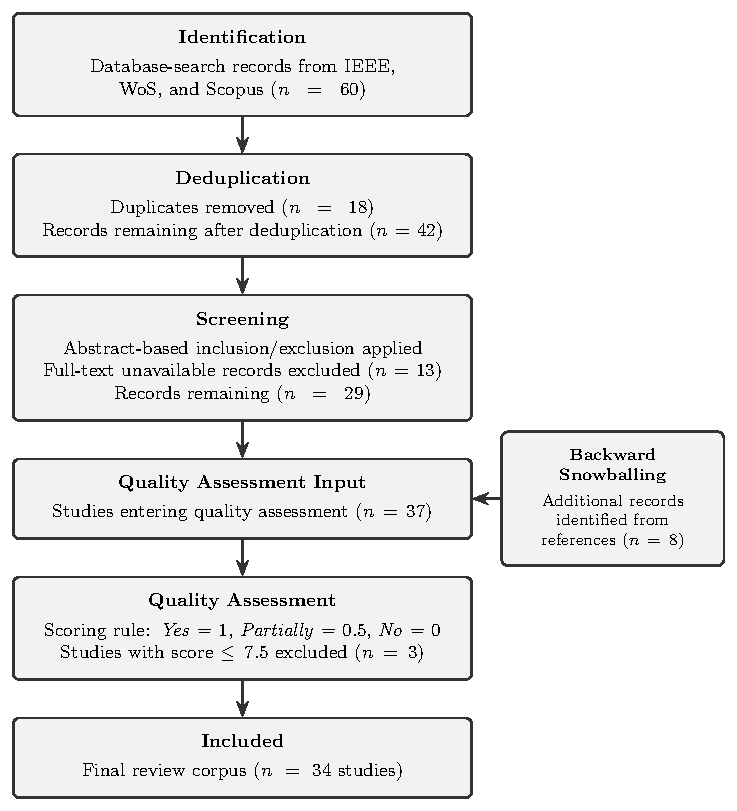
\includegraphics[width=0.60\textwidth]{prisma_flow_diagram.pdf}
\caption{Study selection flow from database retrieval, screening, backward snowballing, and quality assessment.}
\label{fig:prisma}
\end{figure}

\subsection{Search Strategy and Eligibility}

The search strategy combined terminal-context, method, and performance terms. Searches were run on February 27, 2026 in IEEE Xplore, Web of Science, and Scopus, with backward snowballing through Zotero. A preserved Parsifal export in the working archive lists source-level imports of 12 records from IEEE Digital Library, 20 from Web of Science, and 22 from Scopus, plus 8 additional records identified via Zotero-supported backward snowballing. Because these source-level import counts were preserved in a separate working snapshot, the PRISMA flow reported below remains the auditable basis for the screening and retention totals used in this manuscript. The preserved Boolean core of the protocol was:

\begin{quote}
\footnotesize
("agribusiness logistics" OR "cross-docking" OR "dock doors" OR "gates" OR "terminal logistics" OR "truck appointment system" OR "truck arrivals" OR "yard management" OR "yard trucks")\\
AND\\
("dynamic scheduling" OR "heuristic" OR "machine learning" OR "optimization" OR "predictive-reactive scheduling" OR "real-time scheduling" OR "reinforcement learning" OR "resource allocation" OR "simulation")\\
AND\\
("bottleneck reduction" OR "congestion reduction" OR "delay reduction" OR "dock utilization improvement" OR "makespan reduction" OR "operational cost reduction" OR "queue reduction" OR "waiting time reduction")
\end{quote}

Table~\ref{tab:search-audit} records the source-level execution details that remain recoverable from the current workspace and companion materials.

\begin{table}[t]
\caption{Source-level search execution details preserved for retrospective audit.}
\label{tab:search-audit}
\footnotesize
\setlength{\tabcolsep}{4pt}
\renewcommand{\arraystretch}{1.15}
\rowcolors{2}{tablealt}{white}
\begin{tabularx}{\textwidth}{>{\raggedright\arraybackslash\bfseries}p{0.18\textwidth} >{\raggedright\arraybackslash}p{0.14\textwidth} >{\raggedright\arraybackslash}p{0.23\textwidth} >{\raggedright\arraybackslash}p{0.18\textwidth} >{\raggedright\arraybackslash}X}
\rowcolor{tablehead}
\textbf{Source} & \textbf{Execution date} & \textbf{Recoverable retrieval scope} & \textbf{Filters applied} & \textbf{Preserved count} \\
IEEE Xplore & February 27, 2026 & Common Boolean query aligned with title/abstract/keyword retrieval; exact interface field tags not preserved. & No temporal filter. & 12 imported records. \\
Web of Science & February 27, 2026 & Common Boolean query aligned with title/abstract/keyword retrieval; exact interface field tags not preserved. & Publication-year filter 2021--2026. & 20 imported records. \\
Scopus & February 27, 2026 & Common Boolean query aligned with title/abstract/keyword retrieval; exact interface field tags not preserved. & Publication-year filter 2021--2026. & 22 imported records. \\
Backward snowballing via Zotero & Same review cycle after database screening & Reference lists of screened papers; no database-specific field syntax applies. & Same inclusion and exclusion rules as the database search. & 8 additional records. \\
\end{tabularx}
\rowcolors{2}{}{}
\end{table}

This common query was aligned with title/abstract/keyword-oriented retrieval, although the exact advanced-search field tags used in each interface were not preserved in the archived materials. Deduplication is auditable only at aggregate level in the current archive: 18 duplicates were removed, leaving 42 records for screening. No additional records were excluded on topical grounds at title/abstract screening; the screening loss came from 13 records whose full texts remained inaccessible despite exhaustive retrieval attempts through institutional subscriptions, CAPES, institutional repositories, and public author pages. This availability-based attrition corresponds to 31.0\% of the post-deduplication set (13/42). Backward snowballing then added eight studies, yielding 37 studies entering quality assessment and a final retained corpus of 34 studies. The pairwise duplicate log and the article-level metadata of the 13 inaccessible full-text records were not preserved in the current workspace.

Backward snowballing inspected the reference lists of the screened papers through Zotero and applied the same inclusion and exclusion rules used in the main search. This step was used to recover antecedent or adjacent studies that fit the review scope but were not returned directly by the database query.

Inclusion required studies to: (i) address dynamic operations, re-optimization, or uncertainty; (ii) focus on terminals, yards, cross-docking systems, or closely analogous logistics contexts; (iii) propose or evaluate a computational artifact for physical resource allocation; (iv) report some form of validation, such as computational experiments, simulation, benchmarking, or case-based analysis; and (v) be published as peer-reviewed journal or conference papers. Exclusion removed non-technical studies, routing-only papers without internal facility bottlenecks, duplicates, inaccessible full texts, and review or conceptual papers. The temporal filter 2021--2026 was applied in Scopus and Web of Science, but not in IEEE Xplore or snowballing, to preserve earlier antecedent works later screened by the same eligibility rules.

\subsection{Quality Assessment}

The protocol used a ten-question quality-assessment checklist. Each item was scored as \textit{Yes} = 1, \textit{Partially} = 0.5, and \textit{No} = 0, and studies were retained only if the total score was $> 7.5$. The checklist asked:
\begin{enumerate}
\item Is the objective of the modeling clearly defined?
\item Do the results provide useful evidence for real-world applications of truck orchestration in yards, terminals, or analogous logistics contexts?
\item Are the limitations, simplifications, and threats to validity explicitly stated?
\item Does the study test relevant scenarios, events, or operational disruptions?
\item Does the study present validation through experiments, simulation, benchmarking, or computational study?
\item Does the study deliver a clear technical artifact, such as a model, algorithm, architecture, prototype, or system?
\item Does the study explicitly address uncertainty, operational dynamics, and/or real-time re-optimization?
\item Is the proposed method described in sufficient detail for understanding and analysis?
\item Are the decisions, constraints, and objective function clearly presented?
\item Are the logistics focus and the operational context clearly described?
\end{enumerate}

Thirty-seven studies entered quality assessment, three scored $\leq 7.5$, and 34 were retained. Five reviewers used the same screening and extraction form throughout the process. Uncertain inclusion decisions, quality judgments, and later frontier assignments were resolved by joint adjudication so that eligibility and coding criteria remained aligned across the corpus.

\subsection{Extraction and Analytical Synthesis}

For each retained study, the extraction form captured DOI or ISBN, authors and year, application environment, logistics focus, modeling objective, uncertainty treatment, dynamic feature, technical artifact delivered, validation type, events or disruptions tested, performance metrics reported, limitations or gaps, and emerging requirements. This shared structure supported both descriptive synthesis and the interpretive reading developed later in the paper.

The extraction form fed the final analysis in two stages. First, descriptive coding summarized where the literature concentrates in terms of environment, method family, uncertainty treatment, dynamic mode, disruptions, validation strategy, and reported metrics. Second, interpretive coding translated the extraction sheet into the \textit{validity frontier}. Operational pain points were coded primarily from logistics focus and modeling objectives, whereas structural simplifications were coded from assumptions, limitations, and omitted operational factors. These codes were then read through four dimensions: subsystem integration (isolated $\rightarrow$ integrated), uncertainty richness (narrow $\rightarrow$ richer), response mode (offline $\rightarrow$ adaptive), and validation grounding (solver-only $\rightarrow$ simulation or operational evidence). Each study was positioned qualitatively along these four dimensions using the shared extraction form and joint adjudication among reviewers. For example, the predictive-reactive cross-docking model of Nasiri et al. sits in an intermediate position because it addresses truck-arrival uncertainty and rescheduling but remains grounded mostly in constructed instances, whereas the ETA-informed retail case of Modica et al. lies nearer the frontier because it couples adaptive scheduling with case-based operational evidence \cite{nasiri2022,modica2024}. In practical terms, deterministic dock scheduling with isolated resources sits farther from the frontier, whereas ETA-updated or event-stream-driven rescheduling sits nearer. Appendix~\ref{app:audit} summarizes the current preservation status of the review audit trail, Appendix~\ref{app:included} lists the 34 retained studies, and the complete extraction spreadsheet accompanies the manuscript package as \texttt{data\_extraction.xls}.

\section{Findings}

\subsection{Corpus Profile}

The 34 analyzed studies are concentrated in cross-docking centers (12 studies) and container terminals (11 studies). The remaining works address generic logistics systems (4 studies), intermodal rail terminals (2 studies), or do not clearly specify the application environment (5 studies). The corpus also includes cold-chain cross-docks, Physical Internet hubs, and mixed-door configurations \cite{zheng2026,essghaier2023,eti2025}.

\subsection{Evidence Maps}

To preserve study-level traceability without overloading the page, Figs.~\ref{fig:evidence-map-a} and \ref{fig:evidence-map-b} convert the coded extraction sheet into two corpus maps. Figure~\ref{fig:evidence-map-a} shows where the literature concentrates across environments and dominant operational pain points, whereas Fig.~\ref{fig:evidence-map-b} links dynamic sophistication to validation maturity. In both maps, cell values denote study counts rather than performance scores.

\begin{figure}[H]
\centering
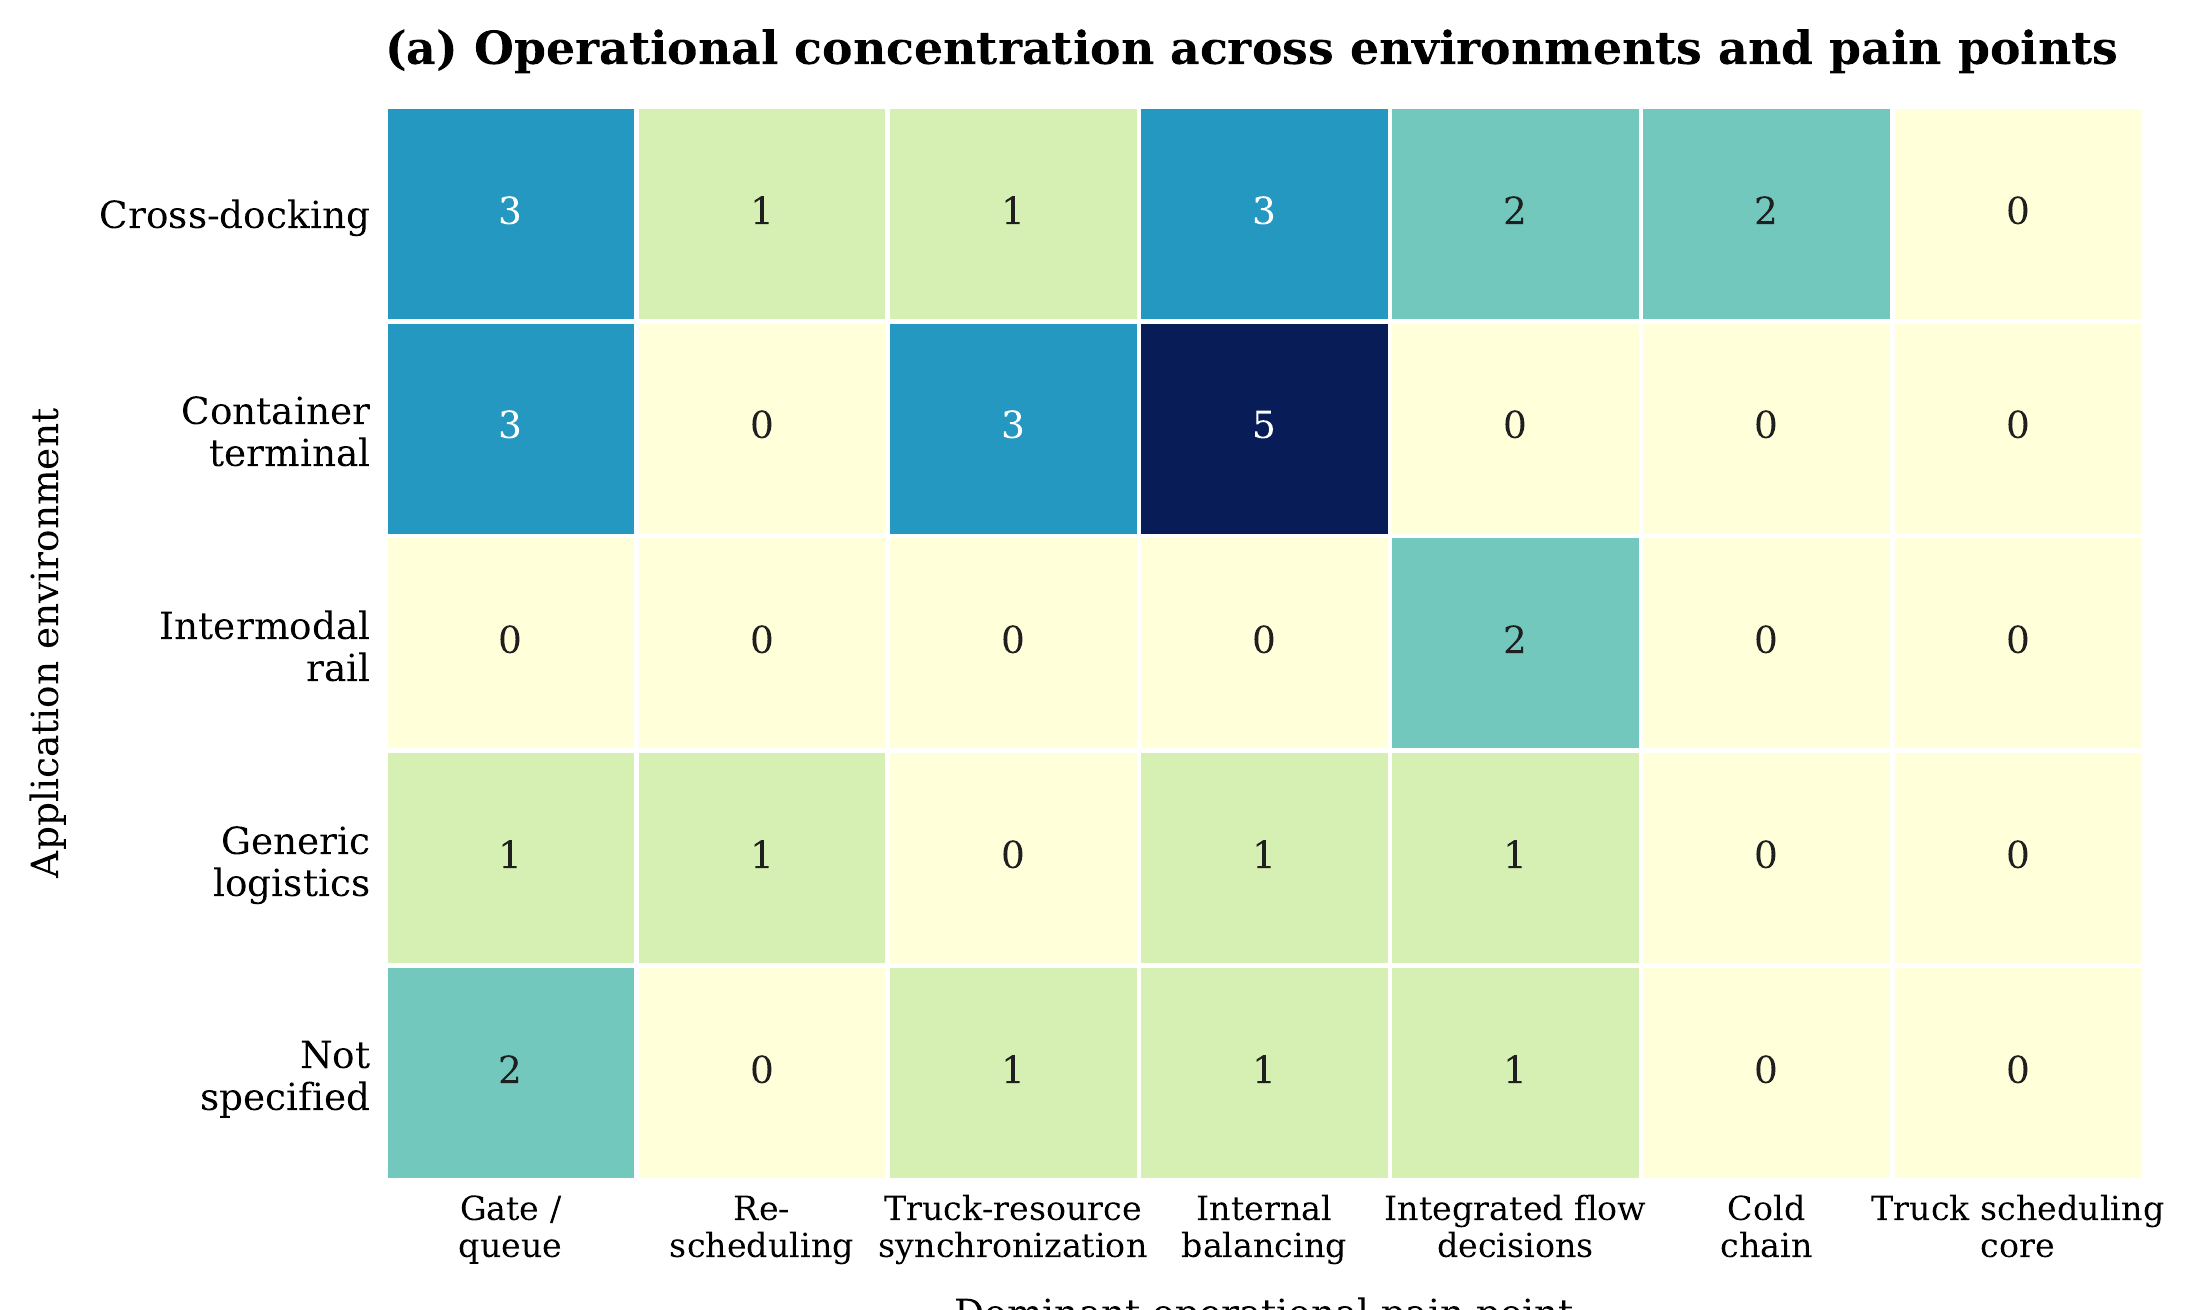
\includegraphics[width=\textwidth]{evidence_map_a.png}
\caption{Operational concentration across application environments and dominant operational pain points. Darker cells indicate that more studies concentrate in the corresponding combination.}
\label{fig:evidence-map-a}
\end{figure}

\begin{figure}[H]
\centering
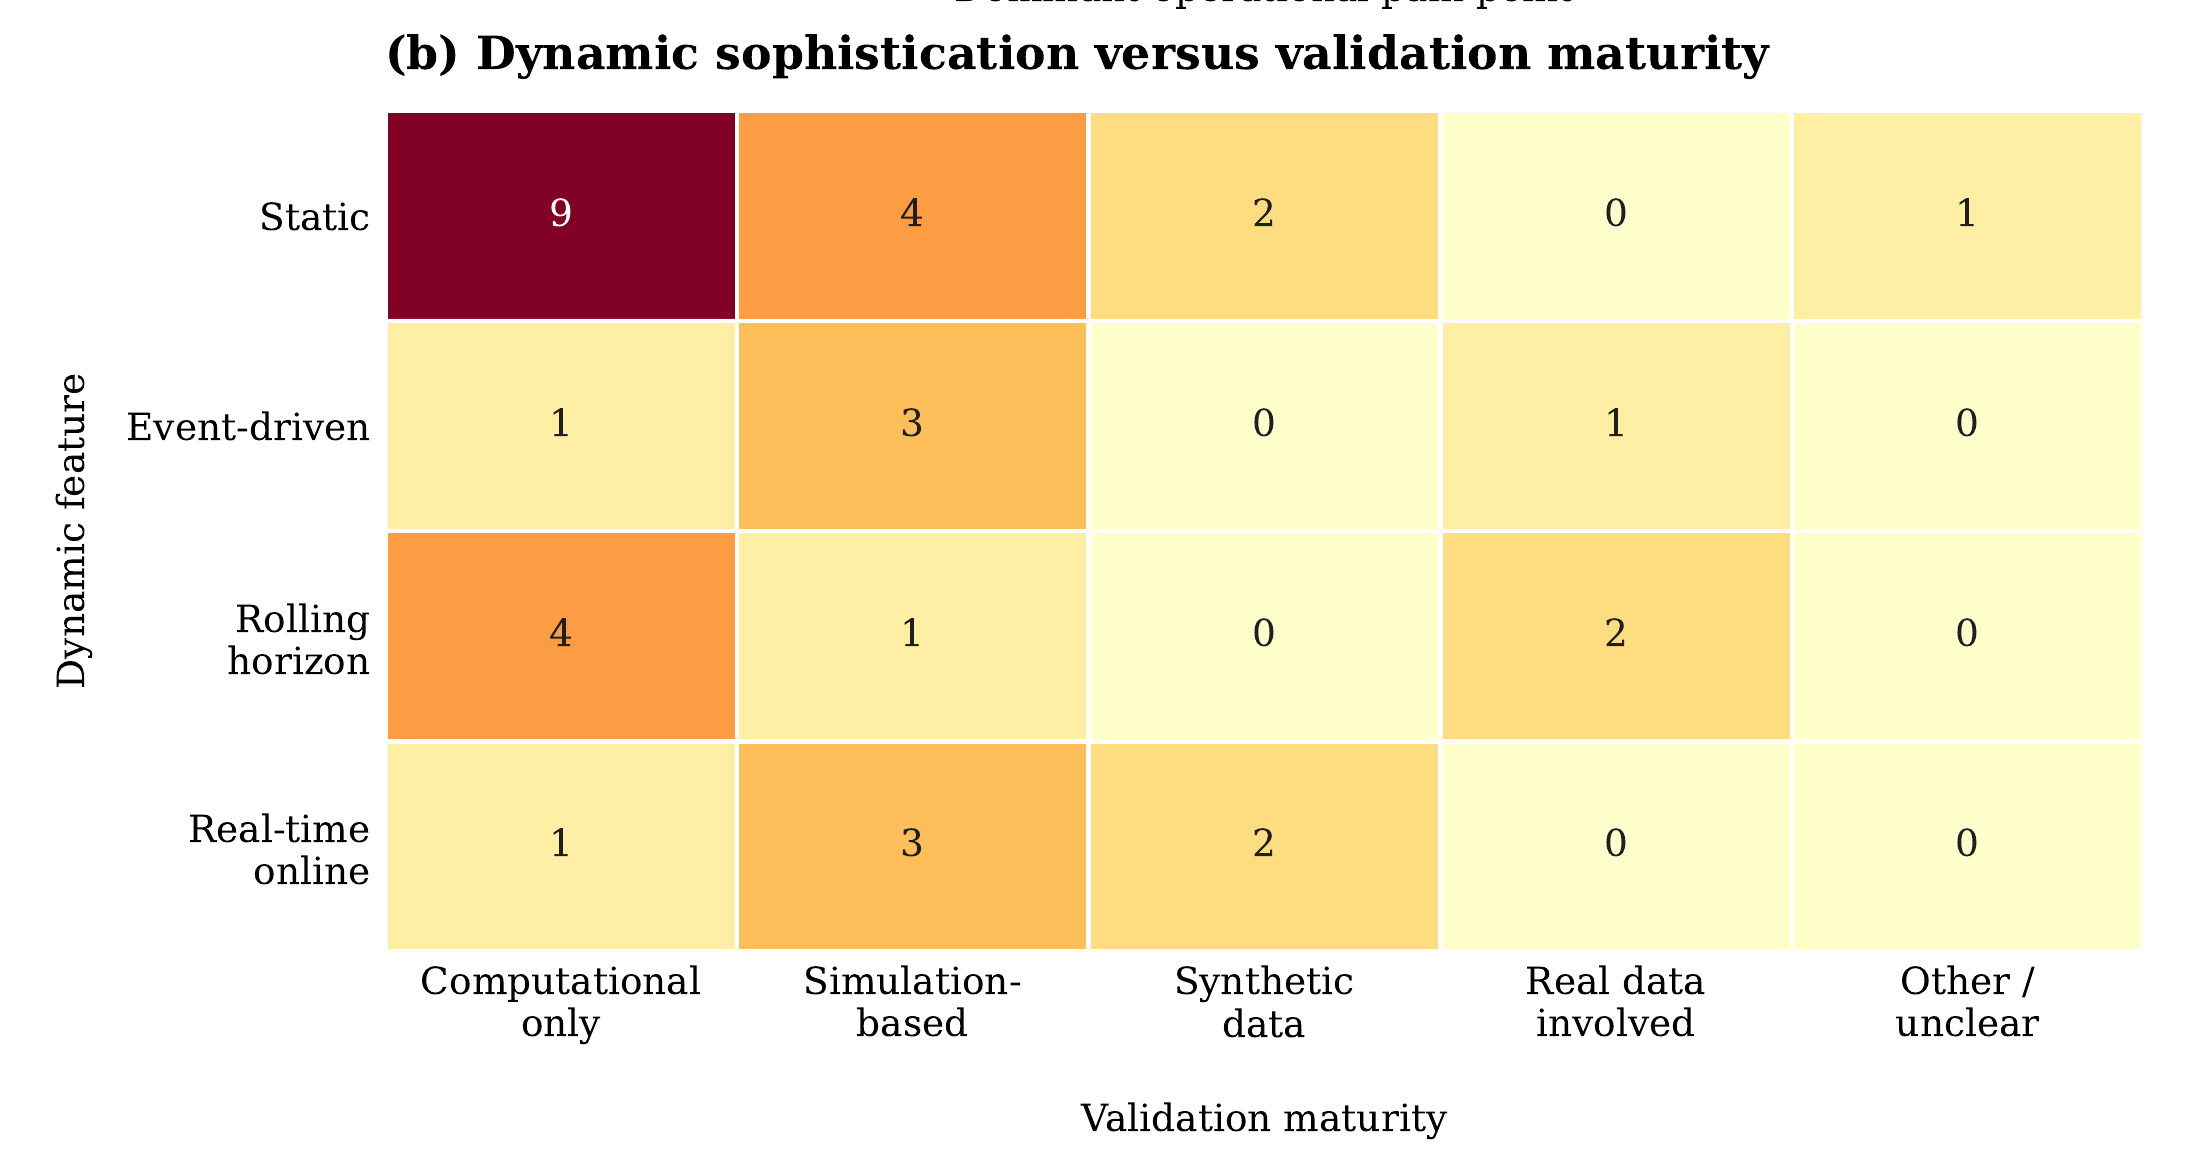
\includegraphics[width=\textwidth]{evidence_map_b.png}
\caption{Dynamic sophistication versus validation maturity. Darker cells indicate that more studies occupy the corresponding combination, exposing the gap between adaptive logic and real-data evidence.}
\label{fig:evidence-map-b}
\end{figure}

The maps make two patterns immediately visible. First, the corpus is concentrated in cross-docking and container-terminal settings, especially around gate congestion, internal balancing, and truck-resource synchronization. Second, adaptive studies still rely mostly on computational experiments and simulation, with little real-data validation. At aggregate level, mathematical programming appears in 24 studies (71\%), metaheuristics in 17 (50\%), hybrid optimization or learning artifacts in 12 (35\%), and simulation or agent-based models in 10 (29\%); stochastic treatment appears in 14 studies (41\%), eight studies (24\%) do not test explicit disruptions, and validation is predominantly computational or simulation-based \cite{dasilva2023,cota2022}.

\subsection{RQ1: Computational Approaches}

Across the corpus, mathematical programming remains the dominant methodological backbone, appearing in 24 studies (71\%), followed by metaheuristics in 17 (50\%), hybrid optimization or learning artifacts in 12 (35\%), and simulation or agent-based models in 10 (29\%). Cross-docking studies more often emphasize temporary inventory, door synchronization, and tardiness control, whereas container-terminal and yard-oriented studies emphasize gate congestion, yard allocation, crane-truck coordination, and uncertain retrieval from storage \cite{nasiri2022,abbas2018,luan2025}. A useful contrast is therefore between MILP-heavy cross-docking formulations and simulation-coupled or agent-based terminal rescheduling, which pursue the same orchestration goal through very different evidence strategies \cite{nasiri2022,abbas2018,torbali2023}. A smaller stream combines optimization with richer signals or auxiliary learning, but even there the main decision engine usually remains an optimization or simulation core rather than end-to-end learning \cite{dasilva2023,luan2025,nogueira2025}.

\subsection{RQ2: Objectives, Dynamics, and Technical Artifacts}

\paragraph{Objectives and Metrics}
Operational objectives remain strongly dominated by temporal control. Across the reviewed studies, schedule adherence, waiting-time reduction, queue mitigation, and makespan minimization appear more often than explicitly environmental or broader systemic objectives. This pattern is visible across cross-docking, container-terminal, and adjacent logistics settings, where models typically seek to reduce tardiness, synchronize truck arrivals and service, or shorten overall completion time \cite{nasiri2022,fonseca2024,eti2025,zheng2026,cekala2015,modica2024,nogueira2025}. Even when cost is modeled explicitly, it is usually decomposed into penalties associated with lateness, queuing, or appointment changes, which makes cost a monetary translation of temporal efficiency \cite{xu2022,xu2021,vahdani2019,wang2023}. Objective-metric alignment is also imperfect: some studies optimize waiting-time, stability, or workload balancing while foregrounding downstream indicators such as $\mathrm{CO_2}$ reduction, throughput, or utilization in the interpretation of results \cite{bouyahia2025,fonseca2024,noh2025,zhang2022}.

\paragraph{Dynamic Features and Artifacts}
At the artifact level, the corpus is transitional rather than fully real-time. Many adaptive studies adopt predictive-reactive or rolling-horizon logic, with ETA updates, appointment reconfirmation, or event-triggered revisions, but continuous online control remains rare \cite{nasiri2022,fonseca2024,torbali2023,dasilva2023,banyai2025,modica2024,xu2022}. A smaller stream combines optimization with richer signals or auxiliary learning, but even there the main decision engine usually remains an optimization or simulation core rather than end-to-end learning \cite{dasilva2023,luan2025,nogueira2025}. Environmental performance therefore appears as an emerging but secondary analytical axis, often embedded in congestion reduction, idling control, or appointment rescheduling rather than treated as an independent optimization objective \cite{bouyahia2025,xu2021,xu2022,zhang2021,zhang2022}.

\subsection{RQ3: Validation Gaps and Practical Applicability}

Validation maturity remains limited. Across the 34-study corpus, 32 studies (94\%) rely on computational experiments, 14 (41\%) include simulation, and only three (9\%) incorporate any real operational data. Solver-oriented validation dominates static or quasi-static settings, while simulation-backed evaluation is the main mechanism used to test adaptive behavior under stochastic arrivals, resource interactions, or event-driven control \cite{cota2022,eti2025,fonseca2024,nogueira2025,vahdani2019,wang2023,zheng2026,abbas2018,li2010,torbali2023,zhang2022}. Synthetic data are used chiefly for benchmark-instance generation, perturbation or scenario generation, and pseudo-operational validation, which strengthens algorithmic comparison but does not close the operational-grounding gap \cite{bouyahia2025,modica2024,noh2025}.

The most recurrent practical limitations follow a recognizable pattern. Many studies isolate one subsystem while leaving upstream and downstream interactions outside the model, treat trucks, cargo, or handling resources as more homogeneous than they are in practice, assume oversized or effectively unlimited temporary buffers, simplify terminal topology and internal travel, or rely on deterministic parameters and highly visible system states \cite{bouyahia2025,noh2025,vahdani2019,cota2022,luan2025,zheng2026}. These simplifications weaken external validity because they suppress spillback, cross-subsystem propagation, and human or infrastructure frictions. In practice, many published orchestration policies remain analytically strong but structurally under-stressed relative to real terminal operations.

\FloatBarrier

\section{Discussion}

The field already offers a broad toolbox for well-bounded scheduling and allocation problems, but deployable orchestration remains less mature. Terminal operations require synchronization across multiple resources, changing truck arrivals, and imperfect information streams \cite{nasiri2022,fonseca2024,abbas2018}, yet many published models still assume simplified disruptions, stable capacities, or centralized information availability \cite{banyai2025,rostami2022,essghaier2023,cota2022}.

\subsection{Analytical Matrix: Pain Points Versus Validity Frontier}

The corpus can be read through two complementary dimensions: recurring logistics pains and the structural simplifications used to keep NP-hard models tractable. Table~\ref{tab:matrix} combines these dimensions and summarizes the main interpretive lens of this review.

\begin{table}[t]
\caption{Analytical matrix linking operational pain points to dominant structural simplifications and external-validity risks. Read each row from left to right: pain point, operational focus, and the simplifying assumption that most threatens external validity.}
\label{tab:matrix}
\footnotesize
\setlength{\tabcolsep}{4pt}
\renewcommand{\arraystretch}{1.15}
\rowcolors{2}{tablealt}{white}
\begin{tabularx}{\textwidth}{>{\raggedright\arraybackslash\bfseries}p{0.22\textwidth} >{\raggedright\arraybackslash}p{0.25\textwidth} >{\raggedright\arraybackslash}X}
\rowcolor{tablehead}
\textbf{Pain point} & \textbf{Operational focus} & \textbf{Dominant simplification and validity risk} \\
Gate congestion and external queues & Protect appointments, reduce idling, and prevent entrance overload. & Gate operations are often modeled apart from the yard and quay, so queue relief may disappear once internal congestion propagates. \\
Disruption-driven rescheduling & Repair obsolete plans after delays, uncertainty release, or workload shifts. & ETA-based disturbance sets are usually narrow, so schedule stability can collapse under coupled events or stale data. \\
Truck-resource synchronization & Prevent truck queues and crane, forklift, or labor idleness. & Identical resources, ignored transfer times, and simplified topology can overstate the level of synchronization that is actually attainable. \\
Internal balancing in yard or cross-dock & Prevent overflow, re-handlings, uneven temporary inventory, and low yard utilization. & Oversized buffers, homogeneous loads, or restricted equipment moves mask spillback, space scarcity, and shutdown risk. \\
Integrated service-window decisions & Coordinate dock sequencing with routing, transfer distance, or multimodal timing. & Deterministic transfer times and stylized waiting assumptions weaken claims of integrated optimality under heterogeneous operations. \\
Cold-chain scheduling & Limit tardiness, spoilage, and stockout under perishability-sensitive service. & Selective uncertainty and stylized degradation logic can overestimate robustness when spoilage and service variability interact jointly. \\
\end{tabularx}
\rowcolors{2}{}{}
\end{table}

Under this lens, many solutions that appear optimal at the algorithmic level are optimal only inside a sanitized operating environment. Recurring assumptions such as homogeneous loads, negligible transfer times, oversized temporary buffers, or partial uncertainty models create a gap between solver success and operational credibility \cite{noh2025,vahdani2019,essghaier2023}. What moves a study nearer the proposed boundary is not simply the presence of dynamic logic, but the combination of broader uncertainty, adaptive updates, subsystem coupling, and validation beyond solver benchmarks.

The matrix also clarifies why methodological sophistication alone is not enough. ETA-informed rescheduling, event-triggered control, and hybrid optimization or learning architectures are meaningful advances, but most are still validated under narrower disturbance spaces and cleaner information environments than real terminals face \cite{dasilva2023,cota2022,xu2022,modica2024,noh2025,luan2025,eti2025}. In that sense, the main dividing line in the literature is less exact versus heuristic optimization and more stylized scheduling performance versus orchestration claims that remain credible when gate, yard, dock, labor, and handling interactions are restored.

This reading also helps position secondary themes such as sustainability and ML. Environmental gains are usually framed as beneficial byproducts of temporal optimization rather than as independently validated trade-offs, while ML typically augments optimization by tuning solvers or exploiting richer event streams instead of replacing the decision core \cite{bouyahia2025,xu2021,xu2022,zhang2021,zhang2022,nogueira2025,dasilva2023,luan2025}. The field is therefore moving toward data-coupled orchestration, but its clearest open need remains operationally grounded validation that tests whether algorithmic gains survive cross-stakeholder data barriers, subsystem coupling, and live execution frictions.

\section{Conclusion and Limitations}

This review maps a field that is rich in scheduling methods but still uneven in subsystem integration, disturbance modeling, and empirical grounding. Across the 34-study corpus, terminal-orchestration research is strongest when solving well-bounded temporal coordination problems and weaker when asked to demonstrate that those gains persist under richer operational complexity. The main contribution of the paper is the exposure of a \textit{validity frontier} for terminal-orchestration research, showing where current approaches remain analytically strong and where they still have narrow operational grounding.

For future work, the evidence points less to new solvers per se than to stronger testbeds and integration assets: shared benchmarks, open synthetic generators tied to realistic signals, digital-twin loops, and studies that connect gate, yard, dock, and handling resources under richer disturbances. For research that claims adaptive or real-time behavior, progress now depends primarily on validation that goes beyond stylized instances and single-site pseudo-operational settings.

Methodologically, the review has limitations. Most importantly, 13 of the 42 post-deduplication records (31.0\%) were excluded because their full texts remained inaccessible even after exhaustive searches through institutional subscriptions, CAPES, institutional repositories, and public author pages. Because the current workspace preserves only the aggregate count, not the definitive article-level list of those records, no source-, topic-, or year-specific sensitivity analysis on that availability loss can yet be performed. The quality cutoff of $> 7.5$ is preserved as a rule, but the study-by-study score matrix and score distribution are not, so threshold-robustness analyses cannot be reproduced retrospectively from the current archive. Because the query was intentionally targeted to terminal, method, and performance terms, relevant studies using different vocabulary may also have been missed. In addition, although the screening and extraction process involved five reviewers using a shared form and joint resolution of disagreements, no formal inter-rater agreement statistic was computed.

\appendix

\section{Audit Trail and Preservation Status}
\label{app:audit}

\begin{table}[h]
\caption{Preservation status of the main review artifacts in the current manuscript package.}
\label{tab:audit-status}
\footnotesize
\setlength{\tabcolsep}{4pt}
\renewcommand{\arraystretch}{1.15}
\rowcolors{2}{tablealt}{white}
\begin{tabularx}{\textwidth}{>{\raggedright\arraybackslash\bfseries}p{0.28\textwidth} >{\raggedright\arraybackslash}p{0.18\textwidth} >{\raggedright\arraybackslash}X}
\rowcolor{tablehead}
\textbf{Artifact} & \textbf{Status} & \textbf{Current evidence in the package} \\
Core Boolean query & Preserved & Reported in Section 2.1 and companion audit notes. \\
Source list, execution date, and imported counts & Preserved & Table~\ref{tab:search-audit} records the three databases, the search date, the source-level counts, and the snowballing additions. \\
Database-specific field tags typed in each interface & Not preserved & The query intent is recoverable, but the exact advanced-search syntax used inside each platform was not archived. \\
Duplicate-pair log & Not preserved & The package preserves the aggregate result of deduplication (18 removals), but not the pairwise duplicate register. \\
Final retained-corpus list & Preserved & Appendix~\ref{app:included} enumerates the 34 included studies. \\
Full extraction spreadsheet & Preserved & The manuscript package includes \texttt{data\_extraction.xls}. \\
Article-level list of the 13 inaccessible full-text records & Not authoritatively preserved & Only the aggregate count is preserved; current Zotero collections allow partial reconstruction of non-retained records, but they do not separate full-text loss cleanly from topical exclusions, duplicate versions, or later replacements. \\
Item-level quality responses, per-study totals, and score distribution & Not preserved & The checklist, answer scale, threshold rule, and retained corpus are preserved, but the complete score matrix is not. \\
\end{tabularx}
\rowcolors{2}{}{}
\end{table}

The most consequential limitation is availability-based attrition. The 13 inaccessible full-text records represent 31.0\% of the post-deduplication set (13/42) and 38.2\% of the size of the final retained corpus (13/34). This is not a topical exclusion but a loss driven by document access. The current workspace therefore supports a transparent report of the magnitude of this bias, but not a definitive appendix listing those 13 studies with article-level metadata. Recovering the original Parsifal screening log remains necessary for a journal-grade audit appendix on full-text loss and for any formal sensitivity analysis around that attrition.

\section{Included Studies in the Retained Corpus}
\label{app:included}

\footnotesize
\begin{longtable}{>{\raggedright\arraybackslash}p{0.18\textwidth} >{\raggedright\arraybackslash}p{0.58\textwidth} >{\raggedright\arraybackslash}p{0.18\textwidth}}
\caption{Studies retained in the final 34-paper corpus.}
\label{tab:included-studies}\\
\toprule
\textbf{Authors (year)} & \textbf{Study title} & \textbf{DOI/ISBN} \\
\midrule
\endfirsthead
\toprule
\textbf{Authors (year)} & \textbf{Study title} & \textbf{DOI/ISBN} \\
\midrule
\endhead
\midrule
\multicolumn{3}{r}{Continued on next page} \\
\endfoot
\bottomrule
\endlastfoot
Jin et al. (2021) & A Dynamic Joint Real-Time Scheduling Strategy of Truck and Yard Crane in Container Terminals & \nolinkurl{10.1109/ICNSC52481.2021.9702168} \\
Li and Li (2010) & Modeling and Simulation of Container Terminal Logistics Systems Using Harvard Architecture and Agent-Based Computing & \nolinkurl{10.1109/WSC.2010.5679030} \\
Li et al. (2009) & Modeling and Simulation of Yard Trailer Dispatching at Container Terminals & \nolinkurl{10.1109/ICAL.2009.5262988} \\
Liu and Liu (2016) & The Hybrid Intelligence Swam Algorithm for Berth-Quay Cranes and Trucks Scheduling Optimization Problem & \nolinkurl{10.1109/ICCI-CC.2016.7862049} \\
Supeno et al. (2015) & Optimum Scheduling System for Container Truck Based on Genetic Algorithm on Spin(Simulator Pelabuhan Indonesia) & \nolinkurl{10.1109/IDM.2015.7516352} \\
Zhang et al. (2022) & Real-Time Scheduling of Autonomous Mining Trucks via Flow Allocation-Accelerated Tabu Search & \nolinkurl{10.1109/TIV.2022.3166564} \\
Zhang et al. (2021) & Scheduling of Autonomous Mining Trucks: Allocation Model Based Tabu Search Algorithm Development & \nolinkurl{10.1109/ITSC48978.2021.9564491} \\
Zouhaier and Ben Said (2016) & An {{Application Oriented Multi-Agent Based Approach}} to {{Dynamic Truck Scheduling}} at {{Cross-Dock}} & \nolinkurl{10.1109/PDCAT.2016.058} \\
da Silva et al. (2023) & Integration of Machine Learning and Simulation for Dynamic Rescheduling in Truck Appointment Systems & \nolinkurl{10.1016/j.simpat.2023.102747} \\
Essghaier et al. (2023) & Fuzzy Multi-Objective Truck Scheduling in Multi-Modal Rail-Road Physical Internet Hubs & \nolinkurl{10.1016/j.cie.2023.109404} \\
Khodashenas et al. (2026) & The Cost and Time Objectives Minimization in Cross-Dock Truck Scheduling of Perishable Goods Considering Uncertainty & \nolinkurl{10.5829/ije.2026.39.02b.16} \\
Luan et al. (2025) & An Efficient Real-Time Railway Container Yard Management Method Based on Partial Decoupling & \nolinkurl{10.1109/TASE.2025.3559241} \\
Movassaghi and Darestani (2022) & Multiple Cross-Docks Scheduling with Multiple Doors Using Fuzzy Approach and Metaheuristic Algorithms & \nolinkurl{10.1007/s40305-021-00362-9} \\
Nasiri et al. (2022) & A Predictive-Reactive Cross-Dock Rescheduling System under Truck Arrival Uncertainty & \nolinkurl{10.1016/j.eswa.2021.115986} \\
Wang et al. (2023) & Flexible Storage Yard Management in Container Terminals under Uncertainty & \nolinkurl{10.1016/j.cie.2023.109753} \\
Xu et al. (2021) & Optimization for a Multi-Constraint Truck Appointment System Considering Morning and Evening Peak Congestion & \nolinkurl{10.3390/su13031181} \\
Bouyahia et al. (2025) & A Novel Truck Appointment System for Container Terminals & \nolinkurl{10.3390/su17135740} \\
Cota et al. (2022) & Integrating Vehicle Scheduling and Open Routing Decisions in a Cross-Docking Center with Multiple Docks & \nolinkurl{10.1016/j.cie.2021.107869} \\
Fonseca et al. (2025) & Stability Approach to {{CDC}} Truck Scheduling Problem under Uncertainty & \nolinkurl{10.1007/s11590-024-02137-6} \\
Kappatos et al. (2025) & Truck Service Optimisation in Port Areas by Comparing Genetic Algorithm and Cuckoo Search Algorithm & \nolinkurl{10.2478/ttj-2025-0030} \\
Movassaghi and Darestani (2021) & Cross-Docks Scheduling with Multiple Doors Using Fuzzy Approach & \nolinkurl{10.48295/ET.2020.79.3} \\
Sha et al. (2021) & Simulation Model to Determine Ratios between Quay, Yard and Intra-Terminal Transfer Equipment in an Integrated Container Handling System & \nolinkurl{10.24006/JILT.2021.19.1.001} \\
Torbali and Alpan (2023) & A Multi-Agent-Based Real-Time Truck Scheduling Model for Cross-Docking Problems with Single Inbound and Outbound Doors & \nolinkurl{10.1016/j.sca.2023.100028} \\
Wang et al. (2025) & Optimizing Expressway Battery Electric Vehicle Charging and Mobile Storage Energy Truck Scheduling: A Two-Stage Approach to Improve Photovoltaic Generation Utilization & \nolinkurl{10.1016/j.energy.2025.135145} \\
Zheng et al. (2026) & Truck Scheduling Optimization at a Cold Chain Cross-Docking Terminal Considering Uncertainties and the Door-Mixed Service Mode & \nolinkurl{10.1016/j.eswa.2025.129849} \\
Abbas et al. (2018) & A Constrained Fuzzy Knowledge-Based System for the Management of Container Yard Operations & \nolinkurl{10.1007/s40815-018-0448-9} \\
Cekała et al. (2015) & Truck Loading Schedule Optimization Using Genetic Algorithm for Yard Management & \nolinkurl{10.1007/978-3-319-15702-3_52} \\
Vahdani and Shahramfard (2019) & A Truck Scheduling Problem at a Cross-Docking Facility with Mixed Service Mode Dock Doors & \nolinkurl{10.1108/EC-08-2018-0355} \\
Xu et al. (2022) & Dynamic Appointment Rescheduling of Trucks under Uncertainty of Arrival Time & \nolinkurl{10.3390/jmse10050695} \\
Banyai and Trojahn (2025) & Adaptive Real-Time Planning of Trailer Assignments in High-Throughput Cross-Docking Terminals & \nolinkurl{10.3390/a18110679} \\
Eti et al. (2025) & Multi-Door Cross-Dock Scheduling under Flexible Doors Mode and Material Handling Resource Restrictions & \nolinkurl{10.1016/j.cor.2025.107183} \\
Modica et al. (2024) & Integrating Arrival Time Estimation in Truck Scheduling: An Explorative Study in Grocery Retailing & \nolinkurl{10.1080/21693277.2024.2425678} \\
Noh et al. (2025) & Inbound Truck Scheduling for Workload Balancing in Cross-Docking Terminals & \nolinkurl{10.3390/math13152533} \\
Rostami et al. (2022) & Modelling Cross-Docking in a Three-Level Supply Chain with Stochastic Service and Queuing System: {{MOWFA}} Algorithm & \nolinkurl{10.3390/a15080265} \\
\end{longtable}

\normalsize

\section*{Declaration of competing interest}

The authors declare that they have no known competing financial interests or personal relationships that could have appeared to influence the work reported in this paper.

\section*{Data availability}

This article is a systematic literature review and does not report a new experimental dataset. The manuscript package includes the retained-corpus extraction spreadsheet (\texttt{data\_extraction.xls}), companion audit notes, and the appendix-level list of included studies. The current package does not yet include the definitive duplicate-pair log, the article-level list of the 13 inaccessible full-text records, or the item-level quality-score matrix; those artifacts require recovery of the original Parsifal workspace used during screening.

\bibliographystyle{elsarticle-num}
\bibliography{artigos_icpr}

\end{document}
